\chapter{系統架構與規劃}
%\label{c:intro}

\lstset{style=mystyle}
本章介紹系統架構與佈局規劃。

\section{系統前半js與html之偵測} 
本研究欲建設一模擬的平台,在此使用者可以打字於一視窗內,此視窗能傳送使用者所打出的文字與計算時間的數據至往後的分析系統裡。(圖3.1)\\\\
%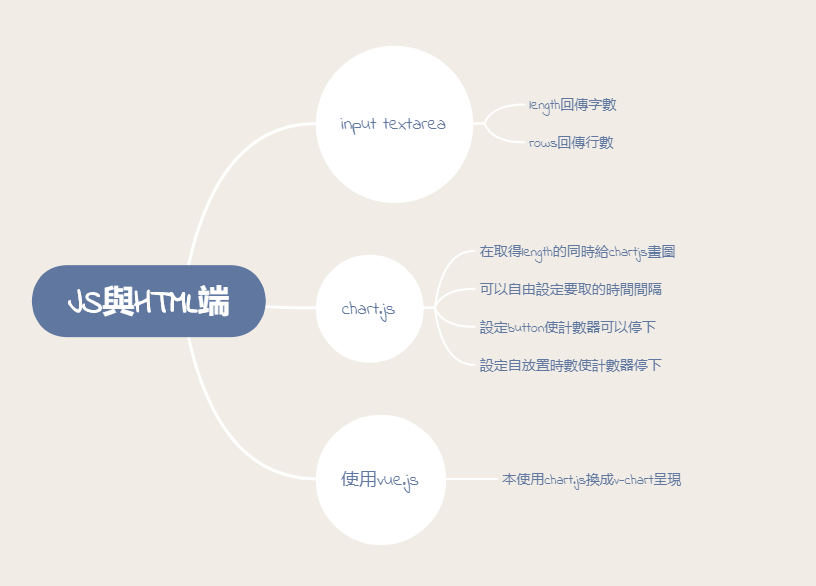
\includegraphics[width = .8\textwidth]{c5C4T4t.png}
\begin{figure}[H] %H为当前位置,!htb为忽略美学标准,htbp为浮动图形
		\centering %图片居中
		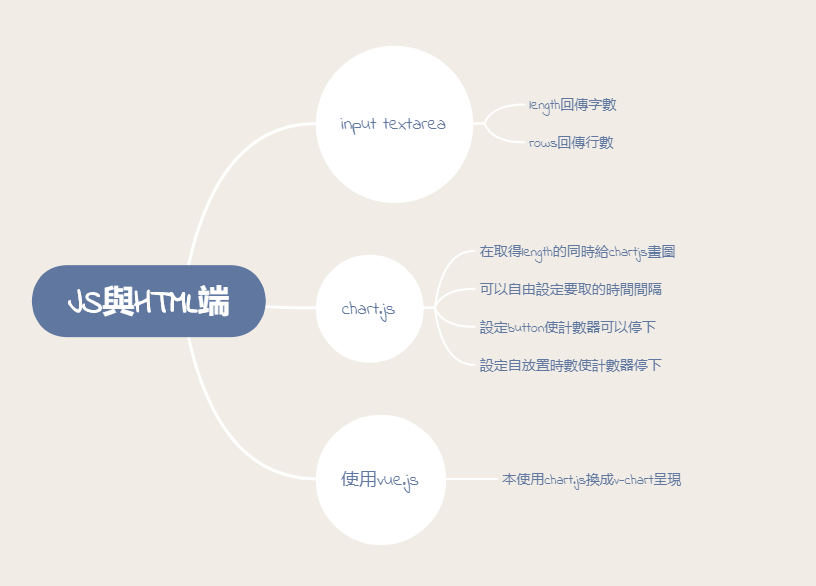
\includegraphics[width=0.7\textwidth]{1.png} %插入图片,[]中设置图片大小,{}中是图片文件名
		\caption{系統前半js與html架構} %最终文档中希望显示的图片标题
		\label{Fig.3.1} %用于文内引用的标签
\end{figure}
\subsection{模擬平台}
在進行觀測同學們的打字程式前,首先要建立一個平台,才能讓使用者在上面進行打字與實驗。
在此使用了一網頁介面進行對使用者打字的前端數據收集,此介面借用了一程式解題平台的網頁介面;在此介面基礎下除了能使用原本的解題,並且能使用本研究的計算字數與時間的功能,並且將種種數據由取間隔相同時間依序存入firebase。
\subsection{輸入}	
\begin{itemize}
	\item textarea的作用\\
	在html網頁中加上textarea的文字框,目的是建立一模擬的打字環境,畢竟本研究討論的是擷取使用者數據與分析其的重要;給使用者平台的管理並不在此研究範圍,因此使用最為簡單明瞭的文字框擷取。
\end{itemize}

\subsection{計算}
\begin{itemize}
	\item 字數與行數的判讀與計算\\
	擷取js程式:

\begin{lstlisting}[caption=js字數與行數的判讀與計算]
function cal_words(){
	var length = document.getElementById("test").value.length;
   //獲取字數數量
	document.getElementById("num").innerHTML = length;
	//回傳給html並顯示
	var rows = document.getElementById("test").value.match(/\r?\n|\r/g).length;
	//抓取換行的字符個數
	document.getElementById("enter").innerHTML =rows;
	//回傳給html並顯示
}
\end{lstlisting}

在使用者打字在作答區時,可以使用javascript語法回傳在文字框的字行數據。
行數據的判斷方法有些許差異,在此我用的是只要使用者打自使用到換行,如enter字符,便會判斷為增加一行。
獲取這些數據後會回傳至html網頁顯示。
\item 時間的判讀與計算\\
我所使用的方法是setTimeout與setInterva函數,但是setTimeout函數只能循環一次,而setInterval()可以不斷循環,故使用setInterval更好。\cite{name20}
也就是說,我加上了固定秒數、時間的基礎上回傳字數資料,相當於固定的時間定時的收集textarea的數據;
如此一來,把時間與數據集中便可以知道時間與使用者打字的關係,進而能夠做到接下來分析的動作。

\end{itemize}
\subsection{輸出}
\begin{itemize}
	\item 圖表\\
	除了能夠獲取實質上的數據數字外,我使用了chart.js與vue.js進行數據繪圖與整理。\cite{name21}(圖3.2)
	\begin{figure}[H] %H为当前位置,!htb为忽略美学标准,htbp为浮动图形
		\centering %图片居中
		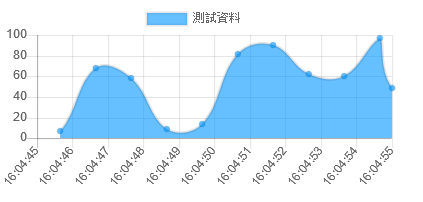
\includegraphics[width=0.7\textwidth]{3.png} %插入图片,[]中设置图片大小,{}中是图片文件名
		\caption{範例圖片} %最终文档中希望显示的图片标题
		\label{Fig.3.2} %用于文内引用的标签
	\end{figure}
此範例圖片是每隔一段時間隨機取一數字並畫成圖,推送至html網頁,他是即時更新的圖表。
而在前頭所提及的setInterval()函數,可與圖表結合,可以更改setInterval()函數所選取的秒數擷取不同時間。所以圖表的輸出為: X軸時間,Y軸字數與行數
	\item 其他功能\\
	除及時推送的圖表外,另加入按鈕可使圖表停止推送。此動作相當於繳交,若要上繳自己所完成的文字檔必定儲存與離開本在工作的頁面,所以圖表與數據計算會停止不再更新與紀錄。
\end{itemize}
\section{系統後半colab分析部分}
	\begin{figure}[H] %H为当前位置,!htb为忽略美学标准,htbp为浮动图形
	\centering %图片居中
	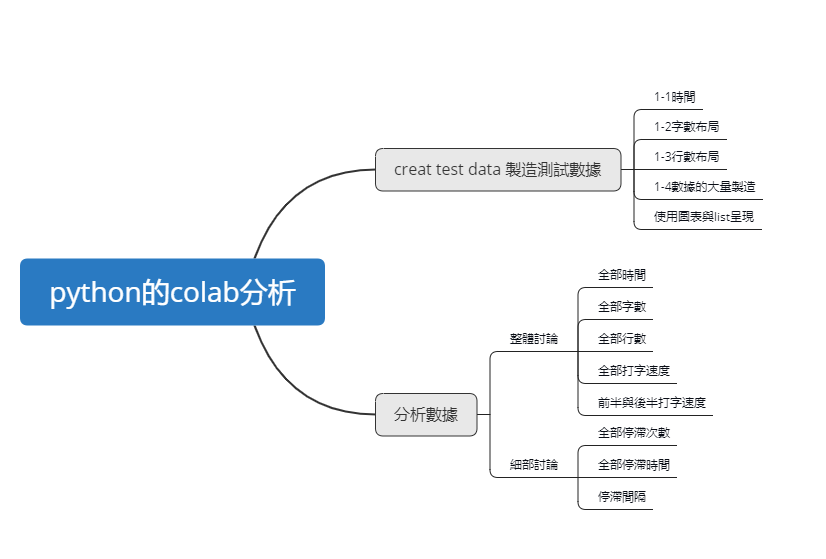
\includegraphics[width=0.7\textwidth]{2.png} %插入图片,[]中设置图片大小,{}中是图片文件名
	\caption{分析系統架構} %最终文档中希望显示的图片标题
	\label{Fig.3.3} %用于文内引用的标签
	\end{figure}
在後半部分本研究換了一種程式語言撰寫,為python。
分析的方向大致為:
1. 某同學做一提的總時間分析,統計大家平均的作答時間
2. 停頓處:若在某處的數據發現停頓,那麼表示這位同學可能在此處卡住
\subsection{製造測試數據}
\subsubsection{討論數據的特徵}
圖(3.4)為在html的程式中執行後的結果,因為是打字數與時間的關係,所以數據自然是漸進式的。佔比面積較大為字數,下部分小的為行數。也就是時間與字行數的關係圖。
但如果數據要一個個採集變不是如此容易,於是面臨測試數據不夠於給之後的分析程式使用,於是便發想也是使用程式製造出類似於測驗結果的數據測試。
	\begin{figure}[H] %H为当前位置,!htb为忽略美学标准,htbp为浮动图形
	\centering %图片居中
	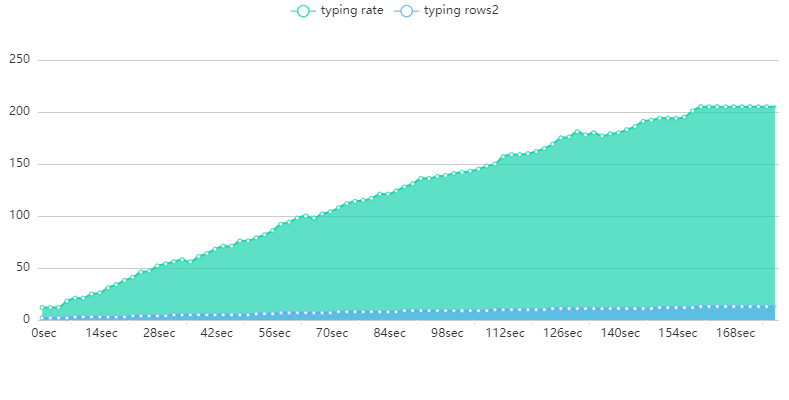
\includegraphics[width=0.7\textwidth]{4.png} %插入图片,[]中设置图片大小,{}中是图片文件名
	\caption{執行結果漸增圖} %最终文档中希望显示的图片标题
	\label{Fig.3.4} %用于文内引用的标签
	\end{figure}
如下討論數據的特徵:
1. 規定時間區間:一個班級同學做同一題目,大家所完成的時間會有差別,可以規定自做的數據時間(ex:15分~1小時),而30分鐘可能是大部分人完成的時間,15分是做得快的,50分以上是做得慢的。
2. 第二欄數據的製造:第二欄是字數的統計,要像是圖(某)中一樣漸進的增加,但是每位同學的字數可能不同,或是停頓的地方可能也不同。它們的字數可能也要設定一個區間。
3. 第三欄為行數,理論上越多字的越多行,但還是必須規定不能生成太多行數。
\subsubsection{規定格式}
觀察圖(3.4)可以知道有好幾組數據在學生打字的時候同步進行計算,而必須規定一數據格式進行傳輸與分析時會較為方便。
這裡為了方便撰寫程式製造類似打字數據的程式,便規定數據必須有三行陣列,也就是3*(時間格數)陣列(圖某),如此陣列的表示數據在作往後的分析或是呈現給使用者看更能靈活地使用。
以下分三部分討論其中數據的構成。
\subsubsection{數據第一部分}
第一部分討論的是時間,網頁程式所抓取的時間是固定的,因此時間的間隔相同。(圖3.5)
	\begin{figure}[H] %H为当前位置,!htb为忽略美学标准,htbp为浮动图形
	\centering %图片居中
	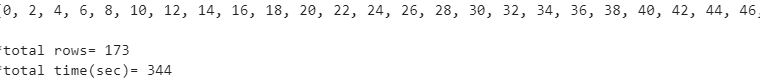
\includegraphics[width=0.7\textwidth]{3_2_1_3.png} %插入图片,[]中设置图片大小,{}中是图片文件名
	\caption{網頁程式執行結果圖} %最终文档中希望显示的图片标题
	\label{Fig.3.5} %用于文内引用的标签
	\end{figure}
每位同學在撰寫時所完成的時間也不相同,在產生數據時規定上下界,如同規定最快完成與最慢完成所需花費的時間。

\begin{lstlisting}[language=Python,caption=python數據第一部分]
data_up = 180
data_down = 500  #可以自行規定秒數區間
random_data = random.randint(data_up,data_down) #這是秒數
r1 = list(range(0,random_data,2)) #r1是第一部分時間陣列的部分
print(r1)
r_row1=len(r1)
r_row2=r1[-1]
print("\n*total rows=",r_row1,)
print("*total time(sec)=",r_row2) #計算random的格數與秒數(秒數為最後一個數據)
\end{lstlisting}
使用random函數進行最大秒數的選擇,後頭的第二與第三數據產生也大量地使用random函數。
\subsubsection{數據第二部分}
第二處可謂最為重要、關鍵與複雜的部份,畢竟是數據最有變化性的部分。
一開始構想的是使用者被網頁觀測到的數據是不停增加,但不會每一段時間增加幅度相同。

\begin{lstlisting}[language=Python,caption=python數據第二部分]
a = random.randint(0,10)
b = random.randint(a,20)
c = random.randint(b,30)
d = random.randint(c,40)
e = random.randint(d,50)
f = random.randint(e,60)
g = random.randint(f,70)
h = random.randint(g,80)
print(a,b,c,d,e,f,g,h)
\end{lstlisting}

如此,此程式所呈現的結果是(8 13 21 34 38 59 64 67),當然每執行一次都不同。
如此撰寫的話,字數會無止盡的增加,在短短時間不可能寫如此快速。只有增加的數據無法反映使用者若是遇到不會的地方的情況,我想加入"若是使用者在思考"的停頓,就是會維持同一個字數許久,而數據不停增加則模擬不出。
打字字數增加,有些地方增加特別快,但也有停頓或是寫錯的地方。如此在打錯的時候使用剪下(ctrl+x)或是倒退(Backspace),所以整體的數據並不會一路平滑的增加,藉由此情狀模擬在作答一個題目數據呈現的變化。

於是在使用者不停增加第二部分字數的基礎上修改至可能停駐思考或是寫錯重來的時候。
新增三個參數分別代表增加、停留、倒退,使用random函數決定使用者可能的三個動作,而在增加與減少的時候數據的變化亮是不等的,此部分也使用random函數實現。(圖3.6)
\begin{figure}[H] %H为当前位置,!htb为忽略美学标准,htbp为浮动图形
	\centering %图片居中
	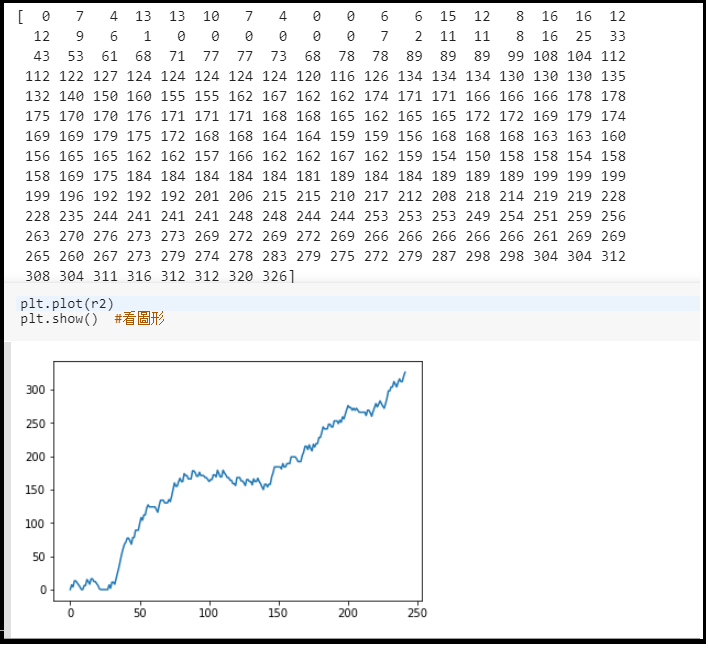
\includegraphics[width=0.7\textwidth]{3_2_1_4.png} %插入图片,[]中设置图片大小,{}中是图片文件名
	\caption{第二部分數據呈現與折線圖} %最终文档中希望显示的图片标题
	\label{Fig.3.6} %用于文内引用的标签
\end{figure}
\subsubsection{數據第三部分}
第三部分為行數 此部分不用著墨太多,雖然第二部分字數與第三部分行數息息相關,但是換行並不用太過關注,或是只要使用原程式碼(js)的監測便會知道使用者換行的時候
第三部分想製造出0,0,0,1,1,1,2,2,2,3,3,3,3,3,3,3,4,4,4,.....如此的陣列漸增關係,但是增加的幅度遠比第二部分的字數還要緩慢許多。(圖3.7)
	\begin{figure}[H] %H为当前位置,!htb为忽略美学标准,htbp为浮动图形
	\centering %图片居中
	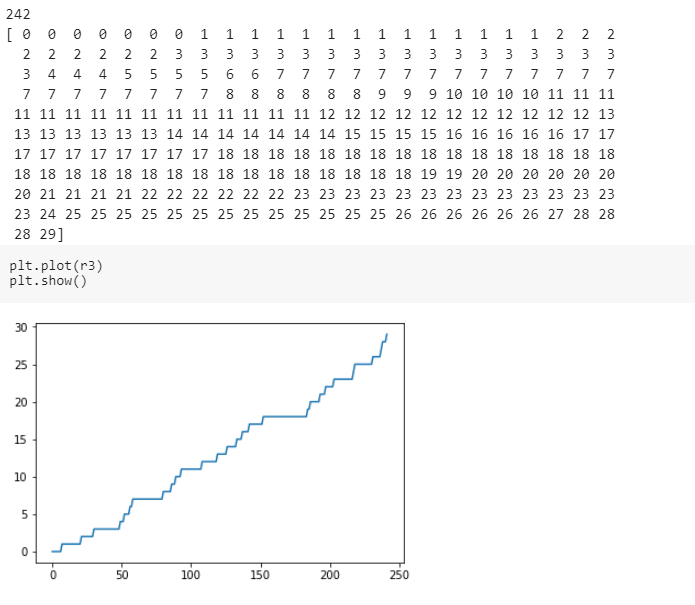
\includegraphics[width=0.7\textwidth]{3_2_1_5.png} %插入图片,[]中设置图片大小,{}中是图片文件名
	\caption{第三部分數據呈現與折線圖} %最终文档中希望显示的图片标题
	\label{Fig.3.7} %用于文内引用的标签
	\end{figure}
\subsection{分析數據部分}
\subsubsection{單組數據整體分析}
\begin{itemize}
	\item 可從最為直觀的記算所有數據的平均速度或是平均字數為基礎,在加上停頓點的分析。因為把數據設計成三個陣列的原因,在分析步驟可以很容易抓到要的數據進行運算。
	\item 在陣列上最容易計算的如:作答時間、做答完畢字數、做答完畢(圖3.8)
	\begin{figure}[H] 
		\centering 
		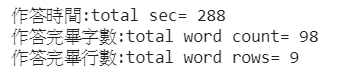
\includegraphics[width=0.7\textwidth]{3_8.png} 
		\caption{整體結果} 
		\label{Fig.3.8} 
	\end{figure}
	然後在往下延伸計算的數據,如:平均做答速度、前半作答速度、後半作答速度;在速度的計算上分兩部分是因為如果只有一個均速可能在比較上會有集大誤差,因此做多個速度的比較數據會更佳。(圖3.9)
	\begin{figure}[H] 
		\centering 
		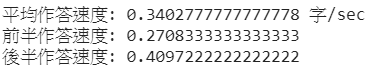
\includegraphics[width=0.2\textwidth]{3_9.png} 
		\caption{整體速度結果} 
		\label{Fig.3.9} 
	\end{figure}
	\item 收集這些速度的數據在之後比較多組,也就是多個同學更能知道每個人的打字速度,除了分析打字的字數外速度也可以加入進行細部分的分析。
\end{itemize}
\subsubsection{單組數據細部分析}
\begin{itemize}
	\item 除了單組數據的整體分析,最總體的數據與平均時間外,打字的停滯點也是至關重要。
	\item 要找出數組中的斷點若是直接觀察是非常容易的,如(圖3.10)
		\begin{figure}[H] 
		\centering 
		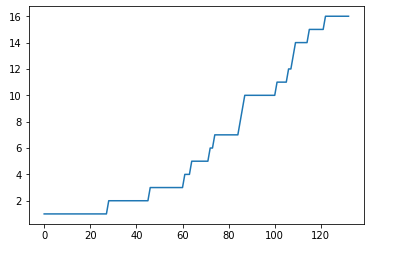
\includegraphics[width=0.7\textwidth]{3_10.png} 
		\caption{示例圖片} 
		\label{Fig.3.10} 
	\end{figure}
	若是看到打字沒有增加,在圖中是平行線段,就代表動作停滯、維持同一字數。
	\item 找出停滯部分本研究所使用方法是,使陣列的後項數據剪去前項數據,並且判斷此數據值若是正數,則判斷增加;若是0,判斷停滯;若是負數,判斷刪除倒退。
	可將此判斷數據化存成另一陣列,在此以下稱trend陣列。\\
	1. 後項減去前項為正:打字字數增加,1表示\\
	2. 後項減去前項為零:打字字數不變,0表示\\
	3. 後項減去前項為負:打字字數減少,-1表示\\
	將判斷後1,0,-1的值存入trend陣列,故此陣列為三個元素組成,且比原本數據的陣列值少一,因為trend陣列是原陣列間隔中的差分。(圖3.11)
		\begin{figure}[H] 
		\centering 
		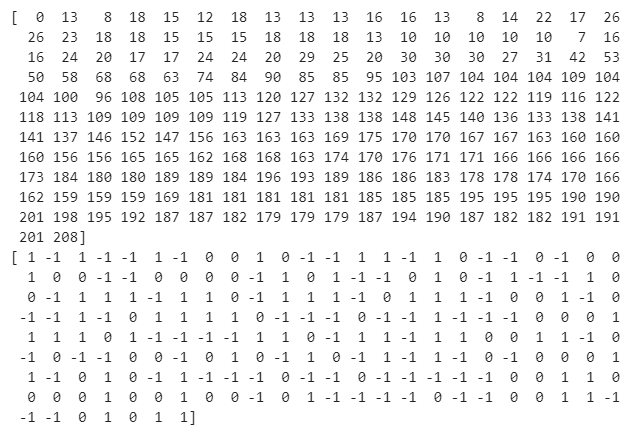
\includegraphics[width=0.7\textwidth]{3_11.png} 
		\caption{trend陣列輸出} 
		\label{Fig.3.11} 
	\end{figure}
	上半部陣列為原數據的陣列,字數遞增;下半部為使用1,0,-1判斷產生的trend陣列。
	如此便很清楚的看出,0是使用者停下的部分,之後能從0所停頓的時間長度,或是停頓所發生的次數判斷分析。
	\item 除了把trend陣列顯示外,若能畫圖更能掌握此陣列數據的特徵。(圖)點狀圖
	\begin{figure}[H] 
		\centering 
		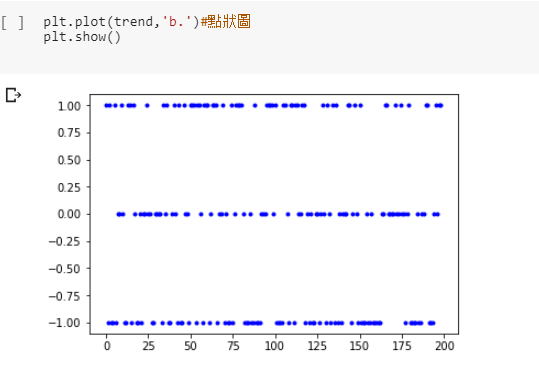
\includegraphics[width=0.7\textwidth]{3_12.png} 
		\caption{trend點狀圖} 
		\label{Fig.3.12} 
	\end{figure}
	(圖)圓餅圖
	\begin{figure}[H] 
		\centering 
		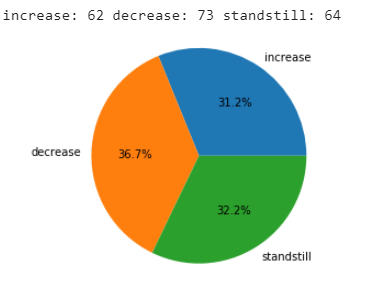
\includegraphics[width=0.7\textwidth]{3_13.png} 
		\caption{trend圓餅圖} 
		\label{Fig.3.13} 
	\end{figure}
\item 製做點狀圖或是圓餅圖可以顯示使用者停頓、打字或是刪除的密集程度。不過此處若是希望只看停頓處的地方,於是在多新增一個新的陣列,以下稱trend2。trend2是把0的元素抓出,把0換成1;因此trend2數據便只有0與1數值。
\item 部分程式:
\begin{lstlisting}[language=Python,caption=python數據trend2]
#len(trend)#trend的隔數 大約表示時間的1/2
trend2=np.zeros(len(trend),int)
for j in range (0,len(trend2)):
	if (trend[j]!=0):
		trend2[j]=0
	else :
		trend2[j]=1
print(trend)
print(trend2)#trend2是trend的停頓部分
\end{lstlisting}
將trend與trend2顯示(圖3.14)
	\begin{figure}[H] 
	\centering 
	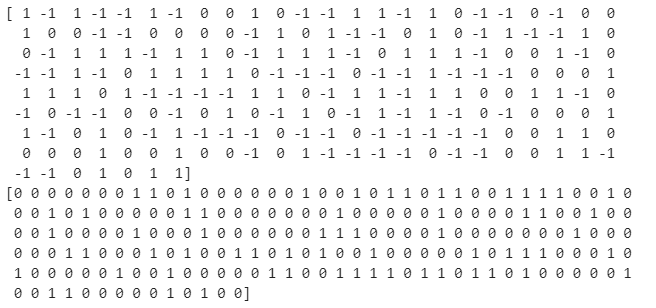
\includegraphics[width=0.7\textwidth]{3_14.png} 
	\caption{trend2輸出} 
	\label{Fig.3.14} 
\end{figure}
\newpage
如此只剩0與1兩個元素的trend2陣列畫成柱狀圖觀察,如同條碼的形狀。(圖3.15)其中線條就是使用者停頓處。
	\begin{figure}[H] 
	\centering 
	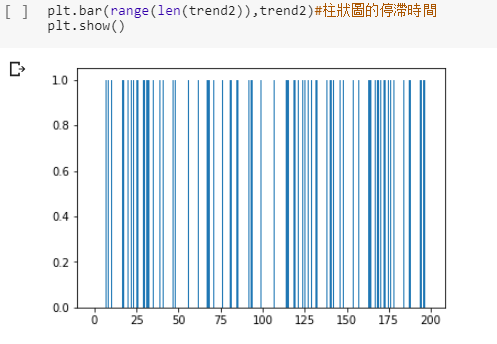
\includegraphics[width=0.7\textwidth]{3_15.png} 
	\caption{trend2條碼狀方圖} 
	\label{Fig.3.15} 
\end{figure}
\item 最後一個圖做分區的統計,這裡計算trend2陣列1的出現次數,並且做分區的統計次數。
分區的分法是察看trend2的全部元素個數,並且分成五等分,在一個個部分統計停頓的出現次數,例如若有200數據,則第一部份統計1出現個數為0~50組,第二部分統計為50~100,以下類推。(圖3.16)
	\begin{figure}[H] 
	\centering 
	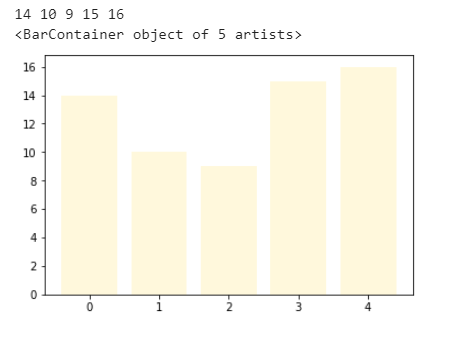
\includegraphics[width=0.7\textwidth]{3_16.png} 
	\caption{trend2分區圖} 
	\label{Fig.3.16} 
\end{figure}
不過如此計算的密度為強制分區,可能無法把密度情況很好的呈現出來,此部份討論於結果部份做詳細討論檢討。
\end{itemize}
\subsubsection{多組數據}
	\begin{figure}[H] 
	\centering 
	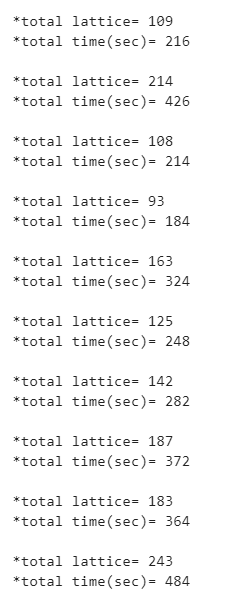
\includegraphics[width=0.5\textwidth]{3_17.png} 
	\caption{多組數據} 
	\label{Fig.3.17} 
\end{figure}
以上分析都是只使用一組數據分析與統計的結果,若要在此基礎上擴增成多數據的分析,則需要進行更多數據的製造與集合分析,所以以上的步驟需要進行多次。
如此進行多次迴圈,此迴全次數可以自行修改。(圖3.17)為設定10次所呈現之全部格數與全部時間。
